% Für Bindekorrektur als optionales Argument "BCORfaktormitmaßeinheit", dann
% sieht auch Option "twoside" vernünftig aus
% Näheres zu "scrartcl" bzw. "scrreprt" und "scrbook" siehe KOMA-Skript Doku
\documentclass[12pt,a4paper,headinclude,bibtotoc]{scrartcl}


%---- Allgemeine Layout Einstellungen ------------------------------------------

% Für Kopf und Fußzeilen, siehe auch KOMA-Skript Doku
\usepackage[komastyle]{scrpage2}
\pagestyle{scrheadings}
\automark[section]{chapter}
\setheadsepline{0.5pt}[\color{black}]

%keine Einrückung
\parindent0pt

%Einstellungen für Figuren- und Tabellenbeschriftungen
\setkomafont{captionlabel}{\sffamily\bfseries}
\setcapindent{0em}

\usepackage{caption}

%---- Weitere Pakete -----------------------------------------------------------
% Die Pakete sind alle in der TeX Live Distribution enthalten. Wichtige Adressen
% www.ctan.org, www.dante.de

% Sprachunterstützung
\usepackage[ngerman]{babel}

% Benutzung von Umlauten direkt im Text
% entweder "latin1" oder "utf8"
\usepackage[utf8]{inputenc}

% Pakete mit Mathesymbolen und zur Beseitigung von Schwächen der Mathe-Umgebung
\usepackage{latexsym,exscale,amssymb,amsmath}

% Weitere Symbole
\usepackage[nointegrals]{wasysym}
\usepackage{eurosym}

% Anderes Literaturverzeichnisformat
%\usepackage[square,sort&compress]{natbib}

% Für Farbe
\usepackage{color}

% Zur Graphikausgabe
%Beipiel: \includegraphics[width=\textwidth]{grafik.png}
\usepackage{graphicx}

% Text umfließt Graphiken und Tabellen
% Beispiel:
% \begin{wrapfigure}[Zeilenanzahl]{"l" oder "r"}{breite}
%   \centering
%   \includegraphics[width=...]{grafik}
%   \caption{Beschriftung} 
%   \label{fig:grafik}
% \end{wrapfigure}
\usepackage{wrapfig}

% Mehrere Abbildungen nebeneinander
% Beispiel:
% \begin{figure}[htb]
%   \centering
%   \subfigure[Beschriftung 1\label{fig:label1}]
%   {\includegraphics[width=0.49\textwidth]{grafik1}}
%   \hfill
%   \subfigure[Beschriftung 2\label{fig:label2}]
%   {\includegraphics[width=0.49\textwidth]{grafik2}}
%   \caption{Beschriftung allgemein}
%   \label{fig:label-gesamt}
% \end{figure}
\usepackage{subfigure}
\usepackage{adjustbox}

% Caption neben Abbildung
% Beispiel:
% \sidecaptionvpos{figure}{"c" oder "t" oder "b"}
% \begin{SCfigure}[rel. Breite (normalerweise = 1)][hbt]
%   \centering
%   \includegraphics[width=0.5\textwidth]{grafik.png}
%   \caption{Beschreibung}
%   \label{fig:}
% \end{SCfigure}
\usepackage{sidecap}

% Befehl für "Entspricht"-Zeichen
\newcommand{\corresponds}{\ensuremath{\mathrel{\widehat{=}}}}

%Für chemische Formeln (von www.dante.de)
%% Anpassung an LaTeX(2e) von Bernd Raichle
\makeatletter
\DeclareRobustCommand{\chemical}[1]{%
  {\(\m@th
   \edef\resetfontdimens{\noexpand\)%
       \fontdimen16\textfont2=\the\fontdimen16\textfont2
       \fontdimen17\textfont2=\the\fontdimen17\textfont2\relax}%
   \fontdimen16\textfont2=2.7pt \fontdimen17\textfont2=2.7pt
   \mathrm{#1}%
   \resetfontdimens}}
\makeatother

%Si Einheiten
\usepackage{siunitx}

%c++ Code einbinden
\usepackage{listings}
\lstset{numbers=left, numberstyle=\tiny, numbersep=5pt}

%Differential
\newcommand{\dif}{\ensuremath{\mathrm{d}}}

%Boxen,etc.
\usepackage{fancybox}
\usepackage{empheq}

%Fußnoten auf gleiche Seite
\interfootnotelinepenalty=1000

%Dateien aus Unterverzeichnissen
\usepackage{import}

\usepackage{url}

\begin{document}

\title{Solarthermie}
\author{Felix Kurtz}
\maketitle

\section{Einleitung}
Bei der Abkehr von fossilen Energieträgern spielt die Sonne als Energiequelle eine zentrale Rolle.
So müssen auch neue Kraftwerke konzipiert werden.
Größtenteils wird dabei auf das bekannte Konzept der Erzeugung von Wasserdampf durch Erhitzen, welcher dann einen Stromgenerator antreibt.
Die Aufgabenstellung ist jedoch, die von der Sonne am Tag gelieferte Energie zu speichern, um auch in der Nacht eine Energieversorgung aufrecht erhalten zu können (vgl. Protokoll \textit{Chemie}).
Hier steht das \textbf{Solarwärmekraftwerk} im Mittelpunkt.
Dabei wird die Sonnenstrahlung mit vielen Spiegeln auf einen Punkt fokussiert.
Dort erhitzt man ein Gas, elches dann wiederum zu einen Wasser zu Wasserdampf erhitzt, aber auch seine Wärme an einen Wärmespeicher abgibt.
Die Spiegel müssen dabei dem Lauf der Sonne folgen, damit der Fokus am gleichen Ort bleibt.

Im DLR SchoolLab ist ein Modell dieses Kraftwerktyps aufgebaut.
Dies soll für die folgenden Messungen benutzt werden.

\section{Aluminium}
Zuerst werden zwei Alu-Platten in den Fokus des Mini-Kraftwerks gehalten und der zeitliche Verlauf der Temperatur notiert.
Die Platten unterscheiden sich eigentlich nur in der Oberflächenbeschaffenheit:
Während die eine metallisch glänzt, ist die andere dunkel beschichtet.
Sie haben eine Größe von $5.5\,\si{\centi\meter}\cdot 6.9\,\si{\centi\meter}=3.8\,\cdot 10^{-3}\si\meter^2$.
Die dunkle Platte wiegt $50.6\,\si\gram$ und die helle $51.5\,\si\gram$
Aluminium hat eine spezifische Wärmekapazität von $c=896\,\si{\joule\per\kelvin\per\kilo\gram}$.
Mit dem gemessenen Anstieg der Temperatur aus Abb. \ref{fig:aluSolar}
\begin{align*}
	\left(\frac{\Delta T}{\Delta t}\right)_\text{D} &= (0.536 \pm 0.021)\,\si{\kelvin\per\second}\quad \text{sowie}\\
	\left(\frac{\Delta T}{\Delta t}\right)_\text{H} &= (0.330 \pm 0.006)\,\si{\kelvin\per\second}
\end{align*}
ergibt sich eine Leistung pro Fläche
\begin{align*}
	\frac{P}{A}=\frac{c\cdot m\cdot\Delta T}{\Delta t}
\end{align*}
für die dunkle Platte von $(6400 \pm 250)\,\si{\watt\per\meter^2}$ sowie für die helle von $(4010 \pm 80)\,\si{\watt\per\meter^2}$.
Geht man davon aus, dass die dunkle Platte $90\%$ der eingestrahlten Leistung absorbiert, beträgt die Strahlungsleistung pro Fläche $(7110 \pm 280)\,\si{\watt\per\meter^2}$.
Dies bedeutet auch, dass die helle Platte nur etwa $56\%$ absorbiert.

Außerdem misst man die Leistung pro Fläche, die bei einem Spiegel ankommt.
Diese liegt bei $990\,\si{\watt\per\meter^2}$.
So wird im Fokus das Licht von etwa 7 Spiegeln gesammelt.
Dies scheint sehr wenig, denn das Spiegelarray besteht etwa aus 100 Spiegeln.
Falls die Messung nicht fehlerhaft war, kann dies daran liegen, dass die Spiegel nicht so gut justiert waren und so der Fokus sehr viel größer als die Fläche, die die beiden Aluminiumplatten einnehmen.
Außerdem wirft die Befestigung Schatten auf die Spiegel.
\begin{figure}[!htb]
	\centering
	\begin{minipage}{0.75\textwidth}	
		\resizebox{\textwidth}{!}{   		
   		% GNUPLOT: LaTeX picture with Postscript
\begingroup
  \makeatletter
  \providecommand\color[2][]{%
    \GenericError{(gnuplot) \space\space\space\@spaces}{%
      Package color not loaded in conjunction with
      terminal option `colourtext'%
    }{See the gnuplot documentation for explanation.%
    }{Either use 'blacktext' in gnuplot or load the package
      color.sty in LaTeX.}%
    \renewcommand\color[2][]{}%
  }%
  \providecommand\includegraphics[2][]{%
    \GenericError{(gnuplot) \space\space\space\@spaces}{%
      Package graphicx or graphics not loaded%
    }{See the gnuplot documentation for explanation.%
    }{The gnuplot epslatex terminal needs graphicx.sty or graphics.sty.}%
    \renewcommand\includegraphics[2][]{}%
  }%
  \providecommand\rotatebox[2]{#2}%
  \@ifundefined{ifGPcolor}{%
    \newif\ifGPcolor
    \GPcolortrue
  }{}%
  \@ifundefined{ifGPblacktext}{%
    \newif\ifGPblacktext
    \GPblacktexttrue
  }{}%
  % define a \g@addto@macro without @ in the name:
  \let\gplgaddtomacro\g@addto@macro
  % define empty templates for all commands taking text:
  \gdef\gplbacktext{}%
  \gdef\gplfronttext{}%
  \makeatother
  \ifGPblacktext
    % no textcolor at all
    \def\colorrgb#1{}%
    \def\colorgray#1{}%
  \else
    % gray or color?
    \ifGPcolor
      \def\colorrgb#1{\color[rgb]{#1}}%
      \def\colorgray#1{\color[gray]{#1}}%
      \expandafter\def\csname LTw\endcsname{\color{white}}%
      \expandafter\def\csname LTb\endcsname{\color{black}}%
      \expandafter\def\csname LTa\endcsname{\color{black}}%
      \expandafter\def\csname LT0\endcsname{\color[rgb]{1,0,0}}%
      \expandafter\def\csname LT1\endcsname{\color[rgb]{0,1,0}}%
      \expandafter\def\csname LT2\endcsname{\color[rgb]{0,0,1}}%
      \expandafter\def\csname LT3\endcsname{\color[rgb]{1,0,1}}%
      \expandafter\def\csname LT4\endcsname{\color[rgb]{0,1,1}}%
      \expandafter\def\csname LT5\endcsname{\color[rgb]{1,1,0}}%
      \expandafter\def\csname LT6\endcsname{\color[rgb]{0,0,0}}%
      \expandafter\def\csname LT7\endcsname{\color[rgb]{1,0.3,0}}%
      \expandafter\def\csname LT8\endcsname{\color[rgb]{0.5,0.5,0.5}}%
    \else
      % gray
      \def\colorrgb#1{\color{black}}%
      \def\colorgray#1{\color[gray]{#1}}%
      \expandafter\def\csname LTw\endcsname{\color{white}}%
      \expandafter\def\csname LTb\endcsname{\color{black}}%
      \expandafter\def\csname LTa\endcsname{\color{black}}%
      \expandafter\def\csname LT0\endcsname{\color{black}}%
      \expandafter\def\csname LT1\endcsname{\color{black}}%
      \expandafter\def\csname LT2\endcsname{\color{black}}%
      \expandafter\def\csname LT3\endcsname{\color{black}}%
      \expandafter\def\csname LT4\endcsname{\color{black}}%
      \expandafter\def\csname LT5\endcsname{\color{black}}%
      \expandafter\def\csname LT6\endcsname{\color{black}}%
      \expandafter\def\csname LT7\endcsname{\color{black}}%
      \expandafter\def\csname LT8\endcsname{\color{black}}%
    \fi
  \fi
  \setlength{\unitlength}{0.0500bp}%
  \begin{picture}(7200.00,5040.00)%
    \gplgaddtomacro\gplbacktext{%
      \csname LTb\endcsname%
      \put(946,704){\makebox(0,0)[r]{\strut{} 20}}%
      \put(946,1111){\makebox(0,0)[r]{\strut{} 40}}%
      \put(946,1518){\makebox(0,0)[r]{\strut{} 60}}%
      \put(946,1925){\makebox(0,0)[r]{\strut{} 80}}%
      \put(946,2332){\makebox(0,0)[r]{\strut{} 100}}%
      \put(946,2740){\makebox(0,0)[r]{\strut{} 120}}%
      \put(946,3147){\makebox(0,0)[r]{\strut{} 140}}%
      \put(946,3554){\makebox(0,0)[r]{\strut{} 160}}%
      \put(946,3961){\makebox(0,0)[r]{\strut{} 180}}%
      \put(946,4368){\makebox(0,0)[r]{\strut{} 200}}%
      \put(946,4775){\makebox(0,0)[r]{\strut{} 220}}%
      \put(1078,484){\makebox(0,0){\strut{} 0}}%
      \put(2032,484){\makebox(0,0){\strut{} 50}}%
      \put(2986,484){\makebox(0,0){\strut{} 100}}%
      \put(3941,484){\makebox(0,0){\strut{} 150}}%
      \put(4895,484){\makebox(0,0){\strut{} 200}}%
      \put(5849,484){\makebox(0,0){\strut{} 250}}%
      \put(6803,484){\makebox(0,0){\strut{} 300}}%
      \put(176,2739){\rotatebox{-270}{\makebox(0,0){\strut{}T [$\si\celsius$]}}}%
      \put(3940,154){\makebox(0,0){\strut{}Zeit [s]}}%
    }%
    \gplgaddtomacro\gplfronttext{%
      \csname LTb\endcsname%
      \put(3586,4602){\makebox(0,0)[r]{\strut{}dunkel (Messwerte)}}%
      \csname LTb\endcsname%
      \put(3586,4382){\makebox(0,0)[r]{\strut{}hell (Messwerte)}}%
      \csname LTb\endcsname%
      \put(3586,4162){\makebox(0,0)[r]{\strut{}dunkel (Fit)}}%
      \csname LTb\endcsname%
      \put(3586,3942){\makebox(0,0)[r]{\strut{}hell (Fit)}}%
    }%
    \gplbacktext
    \put(0,0){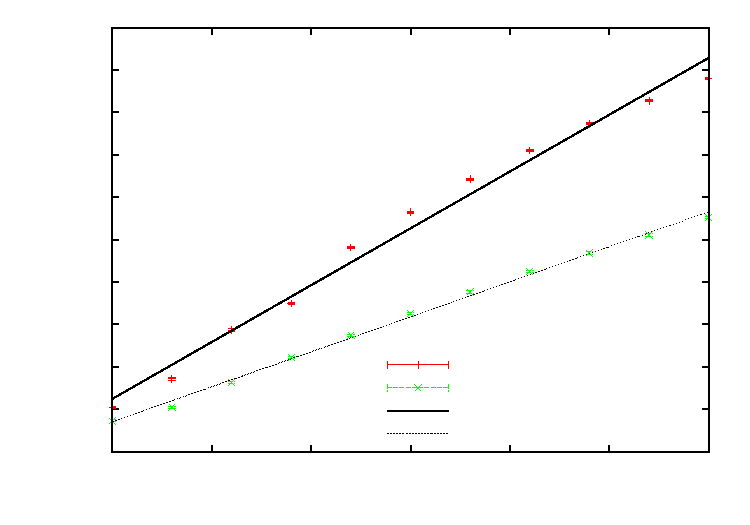
\includegraphics{AluSolar}}%
    \gplfronttext
  \end{picture}%
\endgroup
}
		\caption{Erhitzen der beiden Aluminium-Platten.}
		\label{fig:aluSolar}
   \end{minipage}   
\end{figure}

\section{Wasser vs. Sand}
Nun vergleichen wir die Wärmekapazitäten von Wasser und Sand.
Von beiden Stoffen ist die gleiche Menge (Masse) mit der der gleichen Leistung beschienen worden, sodass die Temperaturerhöhung pro Zeit aus Abb. \ref{fig:wasserSandSolar}
\begin{align*}
	\left(\frac{\Delta T}{\Delta t}\right)_\text{Wasser} &= (0.0566 \pm 0.0024)\,\si{\kelvin\per\second}\quad\text{und}\\
	\left(\frac{\Delta T}{\Delta t}\right)_\text{Sand} &= (0.180 \pm 0.006)\,\si{\kelvin\per\second}
\end{align*}
invers zur spezifischen Wärmekapazität ist: $c_\text{Wasser}=3.18\cdot c_\text{Sand}$.
Wasser hat eine spezifische Wärmekapazität\footnote{\url{https://de.wikipedia.org/w/index.php?title=Spezifische\_W\%C3\%A4rmekapazit\%C3\%A4t&oldid=150986265}} von $4.182\,\si{\kilo\joule\per\kilo\gram\per\meter}$ und somit Sand eine von $1.32\,\si{\kilo\joule\per\kilo\gram\per\meter}$.
Dies bedeutet, dass Sand sich nicht so gut als Wärmespeicher eignet, da er sich schnell erwärmt und sich somit ein hoher Temperaturunterschied zur Umgebung aufbaut, den man durch sehr gute Isolation aufrecht erhalten muss.

\begin{figure}[!htb]
	\centering
	\begin{minipage}{0.75\textwidth}	
		\resizebox{\textwidth}{!}{   		
   		% GNUPLOT: LaTeX picture with Postscript
\begingroup
  \makeatletter
  \providecommand\color[2][]{%
    \GenericError{(gnuplot) \space\space\space\@spaces}{%
      Package color not loaded in conjunction with
      terminal option `colourtext'%
    }{See the gnuplot documentation for explanation.%
    }{Either use 'blacktext' in gnuplot or load the package
      color.sty in LaTeX.}%
    \renewcommand\color[2][]{}%
  }%
  \providecommand\includegraphics[2][]{%
    \GenericError{(gnuplot) \space\space\space\@spaces}{%
      Package graphicx or graphics not loaded%
    }{See the gnuplot documentation for explanation.%
    }{The gnuplot epslatex terminal needs graphicx.sty or graphics.sty.}%
    \renewcommand\includegraphics[2][]{}%
  }%
  \providecommand\rotatebox[2]{#2}%
  \@ifundefined{ifGPcolor}{%
    \newif\ifGPcolor
    \GPcolortrue
  }{}%
  \@ifundefined{ifGPblacktext}{%
    \newif\ifGPblacktext
    \GPblacktexttrue
  }{}%
  % define a \g@addto@macro without @ in the name:
  \let\gplgaddtomacro\g@addto@macro
  % define empty templates for all commands taking text:
  \gdef\gplbacktext{}%
  \gdef\gplfronttext{}%
  \makeatother
  \ifGPblacktext
    % no textcolor at all
    \def\colorrgb#1{}%
    \def\colorgray#1{}%
  \else
    % gray or color?
    \ifGPcolor
      \def\colorrgb#1{\color[rgb]{#1}}%
      \def\colorgray#1{\color[gray]{#1}}%
      \expandafter\def\csname LTw\endcsname{\color{white}}%
      \expandafter\def\csname LTb\endcsname{\color{black}}%
      \expandafter\def\csname LTa\endcsname{\color{black}}%
      \expandafter\def\csname LT0\endcsname{\color[rgb]{1,0,0}}%
      \expandafter\def\csname LT1\endcsname{\color[rgb]{0,1,0}}%
      \expandafter\def\csname LT2\endcsname{\color[rgb]{0,0,1}}%
      \expandafter\def\csname LT3\endcsname{\color[rgb]{1,0,1}}%
      \expandafter\def\csname LT4\endcsname{\color[rgb]{0,1,1}}%
      \expandafter\def\csname LT5\endcsname{\color[rgb]{1,1,0}}%
      \expandafter\def\csname LT6\endcsname{\color[rgb]{0,0,0}}%
      \expandafter\def\csname LT7\endcsname{\color[rgb]{1,0.3,0}}%
      \expandafter\def\csname LT8\endcsname{\color[rgb]{0.5,0.5,0.5}}%
    \else
      % gray
      \def\colorrgb#1{\color{black}}%
      \def\colorgray#1{\color[gray]{#1}}%
      \expandafter\def\csname LTw\endcsname{\color{white}}%
      \expandafter\def\csname LTb\endcsname{\color{black}}%
      \expandafter\def\csname LTa\endcsname{\color{black}}%
      \expandafter\def\csname LT0\endcsname{\color{black}}%
      \expandafter\def\csname LT1\endcsname{\color{black}}%
      \expandafter\def\csname LT2\endcsname{\color{black}}%
      \expandafter\def\csname LT3\endcsname{\color{black}}%
      \expandafter\def\csname LT4\endcsname{\color{black}}%
      \expandafter\def\csname LT5\endcsname{\color{black}}%
      \expandafter\def\csname LT6\endcsname{\color{black}}%
      \expandafter\def\csname LT7\endcsname{\color{black}}%
      \expandafter\def\csname LT8\endcsname{\color{black}}%
    \fi
  \fi
  \setlength{\unitlength}{0.0500bp}%
  \begin{picture}(7200.00,5040.00)%
    \gplgaddtomacro\gplbacktext{%
      \csname LTb\endcsname%
      \put(814,704){\makebox(0,0)[r]{\strut{} 10}}%
      \put(814,1286){\makebox(0,0)[r]{\strut{} 20}}%
      \put(814,1867){\makebox(0,0)[r]{\strut{} 30}}%
      \put(814,2449){\makebox(0,0)[r]{\strut{} 40}}%
      \put(814,3030){\makebox(0,0)[r]{\strut{} 50}}%
      \put(814,3612){\makebox(0,0)[r]{\strut{} 60}}%
      \put(814,4193){\makebox(0,0)[r]{\strut{} 70}}%
      \put(814,4775){\makebox(0,0)[r]{\strut{} 80}}%
      \put(946,484){\makebox(0,0){\strut{} 0}}%
      \put(1922,484){\makebox(0,0){\strut{} 50}}%
      \put(2898,484){\makebox(0,0){\strut{} 100}}%
      \put(3875,484){\makebox(0,0){\strut{} 150}}%
      \put(4851,484){\makebox(0,0){\strut{} 200}}%
      \put(5827,484){\makebox(0,0){\strut{} 250}}%
      \put(6803,484){\makebox(0,0){\strut{} 300}}%
      \put(176,2739){\rotatebox{-270}{\makebox(0,0){\strut{}T [$sicelsius$]}}}%
      \put(3874,154){\makebox(0,0){\strut{}Zeit [s]}}%
    }%
    \gplgaddtomacro\gplfronttext{%
      \csname LTb\endcsname%
      \put(3454,1537){\makebox(0,0)[r]{\strut{}Wasser (Messwerte)}}%
      \csname LTb\endcsname%
      \put(3454,1317){\makebox(0,0)[r]{\strut{}Sand (Messwerte)}}%
      \csname LTb\endcsname%
      \put(3454,1097){\makebox(0,0)[r]{\strut{}Wasser (Fit)}}%
      \csname LTb\endcsname%
      \put(3454,877){\makebox(0,0)[r]{\strut{}Sand (Fit)}}%
    }%
    \gplbacktext
    \put(0,0){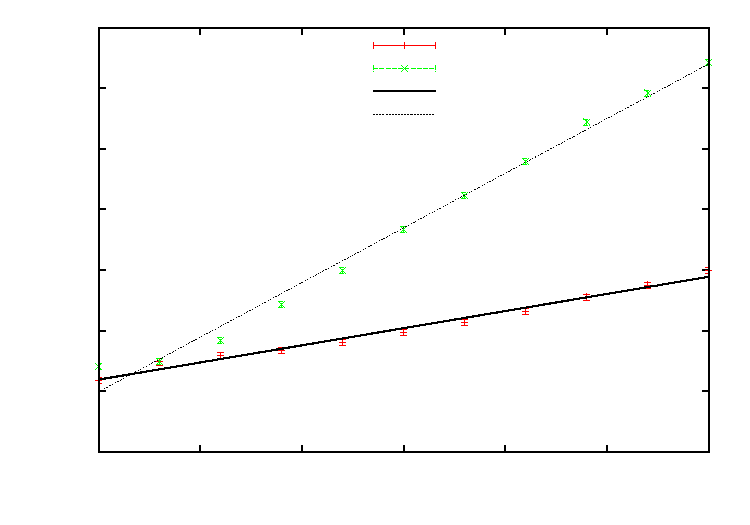
\includegraphics{WasserSandSolar}}%
    \gplfronttext
  \end{picture}%
\endgroup
}
		\caption{Erhitzen von Wasser und Sand im Vergleich.}
		\label{fig:wasserSandSolar}
   \end{minipage}
\end{figure}

\end{document}
